\chapter{Атом}\label{ch:atom}

\epigraph{\emph{Величайшим достижением человеческого гения является то, что человек может понять вещи, которые он уже не в силах вообразить.}}
{Лев Ландау}

Идея об атоме прошла извилистый и местами весьма драматический путь, прежде чем приобрела тот вид, в котором ее изучают сегодня в школах и университетах.
Довольно простая и естественная по своей сути мысль о существовании небольшого числа первоэлементов в итоге привела к совершенно удивительным открытиям.
Все новые и новые факты об атоме, сформировавшие в начале XX века фундамент ядерной физики, поначалу скорее все больше запутывали ученых, нежели вносила ясность.
Оказалось, что знания о микромире попросту нельзя получать и интерпретировать классическим методом - используя интуицию и сравнение с какими-либо привычными объектами вроде стальных шариков или планет Солнечной системы.
Атом оказался чем-то совершенно иным.
Как писал Нильс Бор, ``если ты не шокирован квантовой физикой — ты ее еще не понял''.

Открытие и научное описание процесса деления атомного ядра стало кульминацией всей истории проникновения в тайны атома. 
Именно возможность искусственного расщепления ядер тяжелых атомов позволило освободить огромную энергию, скрытую внутри атома.
Может вызывать некоторый дискомфорт, что это по-настоящему великое открытие впервые было применено именно в военных целях.
Но таков путь истории, и его не изменить.

На протяжении всей книги нам не потребуются ни глубокие факты современной ядерной физики, ни сложный математический аппарат квантовой механики.
Для наших целей будет вполне достаточно общих знаний о строении атома и ядерных реакциях.
Без них было бы крайне тяжело понять, почему те или иные задачи ставились перед физиками и математиками Манхэттенского проекта.
Многие из них были хорошо известны ученым Манхэттенского проекта и с того времени практически не изменились.  
Этих знаний оказалось вполне достаточно для реализации основной его цели - создания ядерного оружия.
Более глубокие факты об атоме были открыты позднее и приводятся здесь лишь в самых общих чертах и только для полноты картины.


\section*{Строение}

Итак, что же такое атом? К настоящему времени известно следующее.
Атом - микроскопическая частица вещества, состоящая из тяжелого ядра, окруженного легкими по сравнению с ним электронами.
Ядро состоит из нуклонов - протонов и нейтронов.
Нуклоны в свою очередь состоят из еще более мелких субатомных частиц: глюонов, кварков и антикварков.
Эти последние частицы интересны в первую очередь тем, что наряду с электронами, вполне могут оказаться действительно \textit{элементарными}, то есть далее неделимыми на более мелкие еще неизвестные науке частицы.
Пока это точно установить не удалось.

\begin{figure}[t!]
   \centering
   \includegraphics[scale=0.5]{images/atom_1}
   \caption{Строение атома гелия: два протона и нейтрона в ядре и два электрона, ``размазанные'' около ядра в облаке формы шарового слоя. Наиболее вероятное местонахождение электронов - пунктирная сфера, но точно локализовать электрон в пространстве невозможно.}
   \label{fig:atom_1}
\end{figure}

На рис. \ref{fig:atom_1} схематически изображен атом гелия.
Он имеет два протона и нейтрона в ядре и два электрона на некотором расстоянии от центра.
В реальности электроны располагаются на очень большом отдалении от ядра - в десятки-сотни тысяч раз большем, чем его диаметр.
Само ядро атома гелия, как и любого другого элемента, в целом устроено довольно просто: протоны и нейтроны упакованы в нем довольно плотно, находясь практически в непосредственной близости друг о друга.

Число протонов в ядре $Z$ называется \textit{зарядовым числом} или \textit{атомным номером}.
Оно однозначно определяет тип химического элемента и его место в периодической таблице элементов: водород - один протон, гелий - два протона и так далее.
Полное количество $A = Z + N$ протонов и нейтронов называют \textit{массовым числом} атома.
Число электронов в атоме совпадает с числом протонов $Z$, что гарантирует его электронейтральность.

Каждый химический элемент, имея фиксированное число протонов, вполне может иметь разное число нейтронов в своем ядре.
Количество нейтронов в ядре практически не влияет на химические свойства атома.
Для одного и того же элемента с разным числом $N$ говорят о его \textit{изотопах}.
Отличаться изотопы одного элемента будут только своей массой, но не свойствами.
Главное, помимо массы, различие разных изотопов одного и того же элемента - их стабильность, о чем подробно рассказано ниже.

Обычно в природе широко распространен какой-то один изотоп каждого химического элемента.
Этот изотоп обнаруживается в подавляющем числе случаев и имеет долгое время жизни.
Остальные изотопы очень редки, либо синтезируются искусственно и имеют очень малое время жизни. 

Например, атом с одним протоном и без нейтронов в ядре представляет собой тот же самый химический элемент, что и атом одним протоном и одним, двумя или тремя нейтронами.
Это все изотопы одного и того же атома водорода: протий \ce{^{1}_{1}H}, дейтерий \ce{^{2}_{1}H}, тритий \ce{^{3}_{1}H} и квадий \ce{^{4}_{1}H}.
Самый легкий из них - протий встречается в природе в $99.98\%$ случаев.

Основной для нас пример - атом урана.
Из 26 известных его изотопов только три встречаются в природе: \ce{^{234}U}, \ce{^{235}U}, \ce{^{238}U}.
Природная смесь добываемого урана содержет в среднем $99.2745\%$ урана-238, $0,72\%$ урана-235 и $0,0055\%$ урана-234
Именно два последних имеют исключительное значение для производства ядерного оружия.
Более тяжелый \ce{^{238}U} найболее распространен в природе ($99.27\%$).
Он устойчив и не может напрямую использоваться как топливо в реакторах или рабочий материал атомной бобмы.
Наиболее ценный и гораздо более редкий \ce{^{235}U} благодаря своим свойствам может сразу быть использован в атомной бомбе, так что .....  

[подробнее о числах для Урана (отдельная секция?)]
[картинка атома урана]
[валентные эоектроны - на внешней оболочке]


\section*{Электронное облако}

Главный и наиболее сложный для понимания факт об электронах в атоме состоит в том, что их точное местоположение указать невозможно.
Они как бы размазаны в пространстве около ядра, образуя \textit{электронное облако} - довольно причудливый трехмерный объект с областями большей и меньшей плотности.

На рис. \ref{fig:atom_1} схематически изображено облако двух электронов атома гелия.
Оно представляет собой сферически симметричную область в пространстве, наиболее плотную в окрестности сферы с центром в ядре атома.
На рисунке это наиболее темная область, выделенная для наглядности пунктиром.
Сами точечные электроны на рисунке - скорее схематическая абстракция, нежели реальные точечные объекты.
Их местоположение не определено точно ни в какой момент времени - они могут находиться практически где угодно, но вероятнее всего - в более темных областях около пунктирной линии.
Подобное поведение физических объектов не встречается нигде в привычных нам наблюдаемых явлениях в обычной жизни.
Оно уникально для микромира. 

Остановимся на этом удивительном факте подробнее.
Принципиально здесь то, что неопределенность положения электрона данном случае отражает не наше субъективное незнание о местонахождении электрона, а объективный факт: положение электрона в пространстве невозможно точно определить никакими инструментами и расчетами.
Первое приходящее на ум объяснение этому факту - мы пока просто не располагаем инструментами необходимой точности, и они когда-нибудь появятся в будущем.
Но это не так.
Невозможность локализовать электрон принципиальна и никак не зависит от наших технических возможностей.

Разница между субъективной и объективной неопределенностью хорошо видна на следующем примере.
Предположим, мы подбрасываем монетку и интересуемся, какой стороной она выпадет.
Если монетка честная, то примерно в половине случаев она будет выпадать орлом, и примерно в половине - решкой.
Подбрасывая монетку, мы действительно заранее не знаем результат и говорим лишь о вероятности выпадения, например, орла.
Но в этом случае мы \textit{все-таки могли бы точно предсказать} результат, если бы знали силу и скорость броска, а также точные турбулентные движения воздуха около монетки.

С электроном все обстоит иначе.
Мы полностью лишены возможности обладания некой дополнительной скрытой информацией вроде движения воздуха вокруг монетки, которая в итоге позволила бы точно определить его местонахождение.
Ученые потратили огромное количество усилий, пытаясь найти подобные \textit{скрытые переменные}, и у них ничего не вышло.
Пришлось признать (и тому есть другие подтверждения), что электрон существует сразу везде, просто где-то с большей вероятностью. 
Распределенное в пространстве состояние - это способ существования электрона в этом мире.
Так все устроено, и ничего с этим не поделаешь. 

Смирившись с невозможностью определить точное положение электрона в пространстве, можно попытаться задаться вопросом о нахождении по крайней мере этой самой вероятности обнаружить его в определенном месте.
Так как в каких-то областях шанс обнаружить электрон выше, то должна быть возможность как-то это количественно описать.
Это, конечно, будут не точные координаты электрона, но уже и не полная неопределенность.

Для описания такого рода частичных неопределенностей в математике используются \textit{плотности распределения вероятностей} - функции, принимающие б'ольшие значения там, где вероятность должна быть выше (подробнее о плотностях см. главу….).
Таким образом, в нашем случае можно сказать, что электрон (даже один единственный!) \textit{распределен} в пространстве так, что его более вероятно обнаружить там, где значение его плотности распределения выше.
С визуальной точки зрения электронное облако электрона оказывается плотнее там, где больше его функция распределения (см. рис. \ref{fig:atom_1}).


Итак, мы связали нашу новую интуицию о положении электрона в пространстве с конкретным математическим объектом - функцией распределения вероятностей. 
Откуда же можно ее получить?
Оказывается, это вполне возможно сделать точно, решив специальное уравнение - уравнение Шреддингера  (\ref{eq:schroedinger_1}), подробнее о котором рассказано ниже.

Плотность вероятности обнаружения электрона в пространстве принято еще называть его \textit{орбиталью}.
Таким образом, математически, орбиталь является одним из решений уравнения Шреддингера.

Сделаем еще несколько замечаний относительно визуализации электронного облака, которое может быть довольно сложным трехмерным объектом.
График функции его плотности находится в четырехмерном пространстве (три пространственные координаты и еще одна ось для значений плотности), и представить его себе довольно проблематично.
Но если электронное облако, например, сферически симметрично, то о полной функции распределения вероятностей вполне можно судить по ее радиальной составляющей, то есть по ее зависимости от $r$ - расстояния до центра атома.
Так, например, для рассмотренного выше атома гелия радиальная составляющая плотности вероятности изображена на рис. (\ref{fig:radial_prob})).

\begin{figure}[t!]
   \centering
   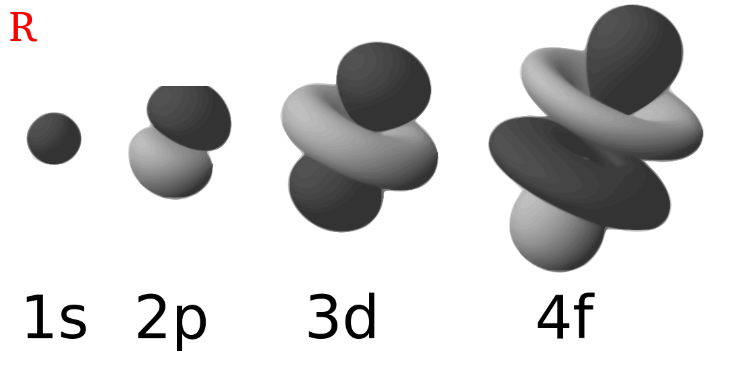
\includegraphics[scale=0.9]{images/electron_clouds_1}
   \caption{Различные виды электронных облаков.}
   \label{fig:electron_clouds_1}
\end{figure}

Иногда, желая придать положению электрона хоть какую-то конкретику, используют геометрическое представление орбитали - поверхность в пространстве, на которой плотность распределения вероятности имеет постоянное значение.
Значение выбирается либо максимальное, либо такое, что в ограничиваемой этой поверхностью области электрон может быть найден с вероятностью близкой к 1.

В случае атомов водорода и гелия эти фигуры представляют собой сферу с центром в ядре атома.
Это уже гораздо более наглядные геометрические образы, нежели абстрактные плотности распределения вероятностей.
Однако важно понимать, что они не определяют точные местоположения электрона в пространстве. 
В реальности электроны вовсе не двигаются по своим орбиталям по аналогии с движением планет Солнечной системы по своим орбитам.
Более того, само понятие движения электрона в данном случае весьма условно.
О конкретных координатах электрона, как и о траектории движения электрона по орбитали речи идти не может.

Наконец, электронное облако далеко не всегда имеет шарообразную форму.
Наиболее симметричная форма облака в виде простого шарового слоя как на рисунке \ref{fig:atom_1} может наблюдаться только у атомов водорода и гелия.
У других химических элементов формы электронных облаков гораздо сложнее и даже могут не иметь сферической симметрии.
На рис. (\ref{fig:electron_clouds_1}) изображено несколько примеров не сферически симметричных облаков.
Удивительно, но все эти замысловатые фигуры реализуются как некоторые решения уравнения Шреддингера (\ref{eq:schroedinger_1}).



\section*{Размеры}

Линейные размеры атома определить достаточно сложно из-за описанной выше неопределенности положения его электронов в пространстве.
О размерах атома принято судить либо по наиболее вероятной удаленности его электронов от ядра, либо по половине расстояния между ядрами двух одинаковых атомов в молекуле простого вещества.
В любом случае они неимоверно малы - от $31\cdot 10^{-12}$ (атом гелия) метра до $225\cdot 10^{-12}$ (атом цезия) метра.
Порядком размера атома принято считать величину $1\mbox{\normalfont\AA} = 10^{-10}$ м (ангстрем).
Понять, насколько это мало, можно учтя, что атомов в капле воды примерно $4\cdot 10^{21}$, что вполне сравнимо с числом звезд во Вселенной.

Так как нуклоны в ядре упакованы довольно плотно, то о размере ядра вполне можно судить по размеру одного нуклона - около $0.86\cdot 10^{-15}$ метра (примерно одинаковы для протонов и нейтронов). 
Таким образом, ядро в десятки - сотни тысяч раз меньше, чем весь атом.
Так, для простейшего атома водорода с диаметром порядка $53\cdot 10^{-12}$ метра и единственным протоном в ядре, электрон удален от центра на расстояние примерно в 100000 раз большее, чем само ядро \footnote{%
    Здесь, конечно же, имеется ввиду средняя удаленность электрона от ядра.
    О точном расстоянии до ядра говорить не приходится.}.
Таким образом, между протоном и электроном, где бы последний ни находился, расположено огромное количество пустоты.

Относительно размеров электрона даже в настоящее время известно очень немногое.
Последние попытки его определения показали, что оно не превосходит $10^{-20}$ метра.
В настоящее время электрон принято считать \textit{фундаментальной элементарной частицей}, то есть такой, которую пока не удалось разложить на составные частицы и определить ее размер.

В связи с этими числами обычно приводят следующий пример: если ядро увеличить до размеров теннисного мячика, то весь атом увеличится до размеров футбольного стадиона.
Электрон при этом станет не более чем песчинкой, спрятанной где-то в последних рядах стадиона без малейшего шанса его найти.

... переход

Орбитали атомов размазаны в пространстве, и невозможно точно отделить атом от окружающей его пустоты.
Более того, если учесть, что размер электронов пренебрежимо мал, а наиболее вероятные места их пребывания сконцентрированы в тонких слоях около поверхностей максимальной плотности вероятности, то электронному облаку можно не приписывать сколько-нибудь существенного объема.
Атомные ядра также имеют неимоверно малые размеры как сами по себе, так и по сравнению с размерами атомов.
Нуклоны, составляющие ядра, также не плотны, а в свою очередь состоят из более мелких \textit{фундаментальных элементарных частиц}.
Таким образом получается, что мы живем в практически пустом пространстве.


\section*{Масса}


\section*{Заряд}


\section*{Свойства}


\section*{Стабильность и распад}

Итак, атом в целом устроен довольно просто.
Но почему же он стабилен?
Чтобы атом мог существовать сколько-нибудь продолжительное время, между его протонами, нейтронами и электронами должны действовать некоторые силы.
Именно эти силы и делают атом стабильной структурой.
Эти силы не дают частицам, с одной строны, разлететься в разные строны, а с другой - упасть друг на друга.



Как было сказано выше, атомы одного и того же химического элемента всегда имеют фиксированное число протонов, но могут иметь разное число нейтронов. 
Эти обеспечивается разнообразие ...
Главное, помимо массы, различие разных изотопов одного и того же элемента - их стабильность, о чем рассказано ниже.



В среднем число нейтронов для изотопов данного химического элемента не слишком отличается от числа протонов, которое для него определено однозначно.
Число нейтронов у изотопа может быть как меньше, так и больше числа протонов.
В обоих случаях, чем больше эта разница, тем неустойчивее атом становится и тем выше вероятность ему распасться на атомы более легких элементов.
Если число нейтронов отличается от 

Выше было рассказано о неустойчивости разных изотопов и естесственной радиоактивности...
Это явления имеет ключевое значени для искусстевенного расщепления ядра атома...


Стабильность атома определяется через \textit{период полураспада} - время, за которое распадутся ядра 




Простейшим из атомов является атом водорода, обладающий минимальным числом протонов - одним.
Число нейтронов в атоме водорода может быть от нуля до семи, но с ростом их числа ядро становится нестабильным и быстро спонтанно распадается.
Так, у трития - изотопа водорода с тремя протонами, период полураспада составляет около 12 лет, а у квадия с четырьмя протонами - всего $1.4\cdot 10^{−22}$ секунды.
Это же верно для любых атомов.
Нейтроны необходимы, чтобы стабилизировать пытающиеся разлететься протоны, но с ростом их числа атом все-таки теряет стабильность (см. рис. \ref{fig:atom_stability}).


\begin{figure}[t!]
   \centering
   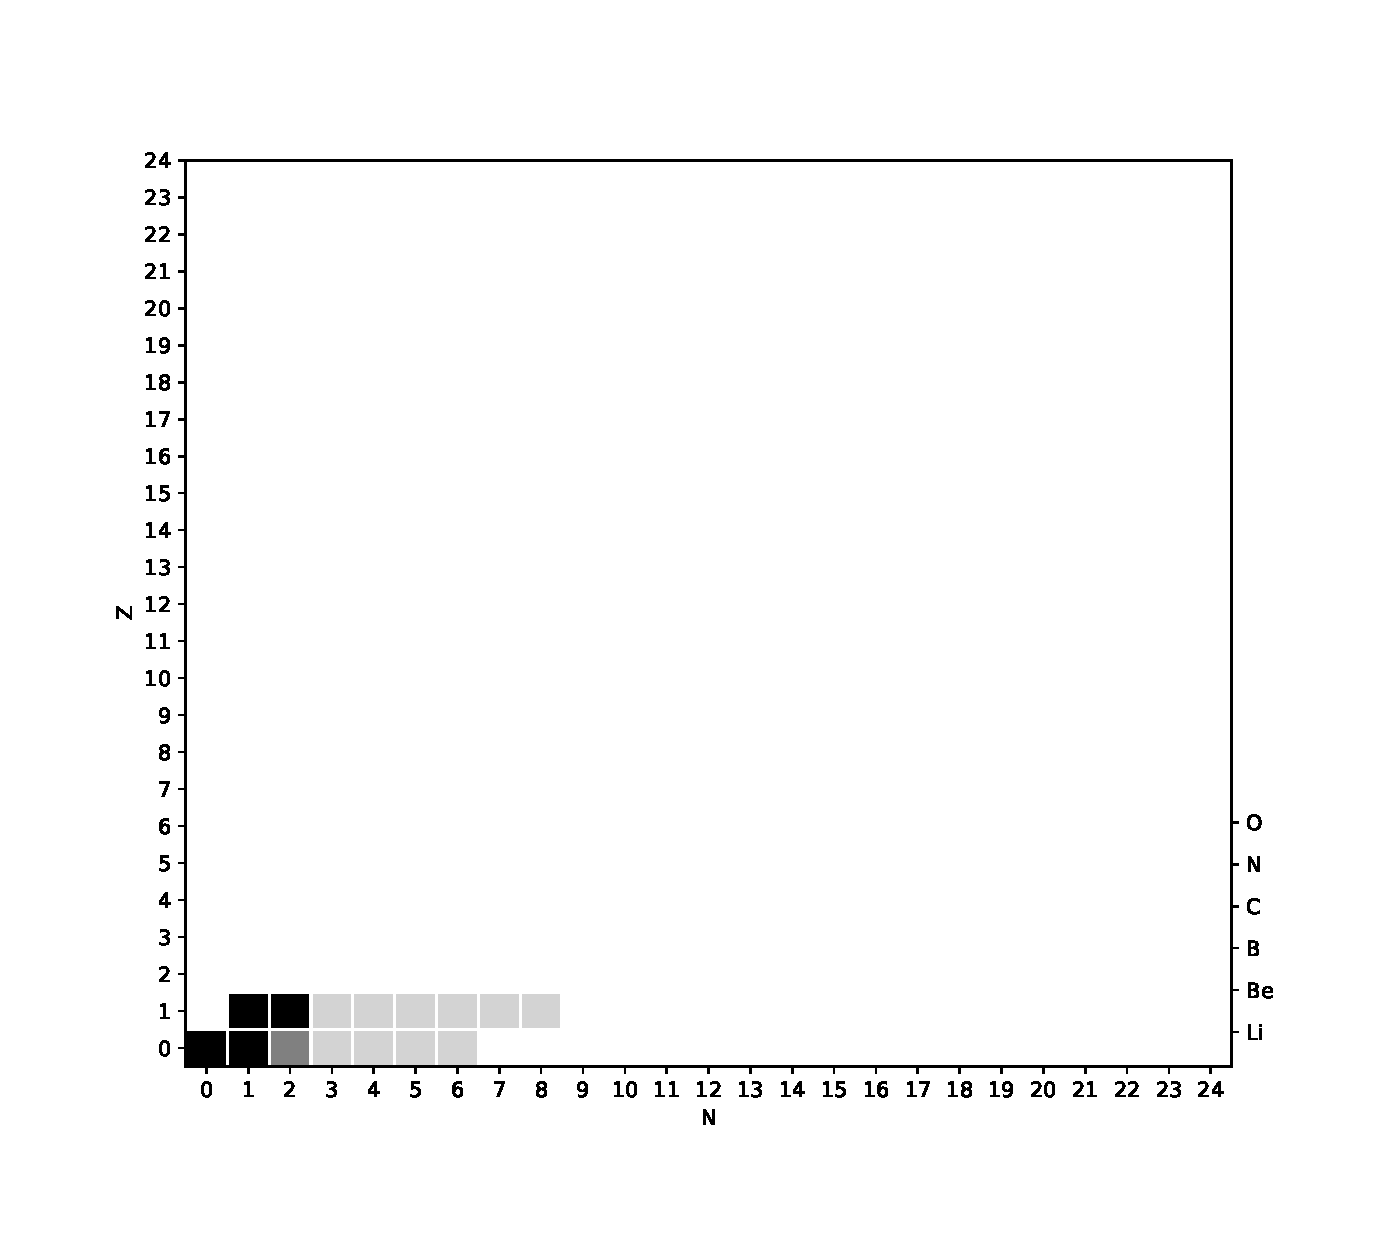
\includegraphics[scale=0.4]{images/atom_stability}
   \caption{Фрагмент диаграммы стабильности атомов химических элементов в зависимости от числа протонов и нейтронов в ядре. Темные клетки - стабильные атомы, светлые - относительно стабильные атомы, живущие от часов до миллиардов лет, пустые - нестабильные атомы, живущие не более малых долей секунд.}
   \label{fig:atom_stability}
\end{figure}




Электроны и протоны являются носителями электрического заряда, нейтроны электрически нейтральны. 
Электроны отрицательно заряжены, протоны - положительно, причем заряд электрона равен заряду протона, а числа электронов и протонов в атоме равны, так что атом оказывается электронейтральным в целом.
Бывает, что атом теряет или приобретает электроны, приобретая таким образом заряд и новое название - ион.
Здесь нас будут интересовать только атомы, не имеющие заряда.

При массе атома от $1.7\cdot 10^{-27}$ кг (атом Водорода-1) до $209.6\cdot 10^{-27}$ кг (атом свинца-208) масса одного электрона составляет всего $9.1\cdot 10^{-31}$ кг.
То есть в ядре сконцентрировано более $99.9\%$ всей массы атома.
Интересно, что кварки, из которых состоят протон, дают менее $2\%$ его массы, основная же часть массы протона приходится на виртуальные частицы.
Нам далее не потребуются столь глубокие субатомные понятия, как кварки и виртуальные частицы. 
Многие из них были открыты и изучены уже после Манхэттенского проекта и никак на него не повлияли. 


\section*{Цепные реакции}

Химические превращения одних веществ в другие происходят только путем перегруппировки атомов между их молекулами.
В процессе химической реакции молекулы исходных веществ отдают или принимают атомы, в результате образуя молекулы новых веществ. 
Сами атомы при этом остаются неизменными.
В этом смысле атом действительно является \textit{наименьшим} носителем химических свойств данного вещества, как и думали древние.

Таким образом, одних простых химических реакций недостаточно, чтобы решить главную задачу алхимии - заставить атомы одного вещества стать атомами другого.
Для того чтобы атомы одного вещества превратились в атомы другого, необходимо более грубое физическое вмешательство - ядерные реакции, в процессе которых ядра атомов взаимодействуют друг с другом или с элементарными частицами.
В результате ядерных реакций тяжелые атомы могут распадаться в более легкие (реакции деления), либо соединяться в еще более тяжелые (реакции синтеза).
Оба этих типа реакций происходят с выделением огромного количества тепла и радиации, что и послужило главной причиной для использования их в военных целях.

------------------------

сколько энергии выделяется при арспаде одного этома...


\section*{Уравнение Шреддингера}

Эта секция ... не важна для общего опнимания ....

УШ - чисто математический объект, причем весьма непростой.

Итак, откуда же можно получить хотя бы вероятность нахождения электрона в заданной области пространства?
Оказывается, она может быть найдена точно как решение уравнения Шреддингера

\begin{equation}\label{eq:schroedinger_1}
\nabla\psi + \frac{2m}{\hbar^2}(E - U(x))\psi = 0.
\end{equation}

Решения этого уравнения $\psi(x)$ комплекснозначны, но физический смысл имеют только их модули. 
Не вдаваясь в технические детали, можно сказать, что уравнение (\ref{eq:schroedinger_1}) дает искомую плотность вероятности обнаружения электрона в точке $x$ как квадрат модуля функции-решения $|\psi(x)|^2$.
Подробнее об уравнении Шреддингера можно почитать в приложении ....

\begin{figure}[t!]
   \centering
   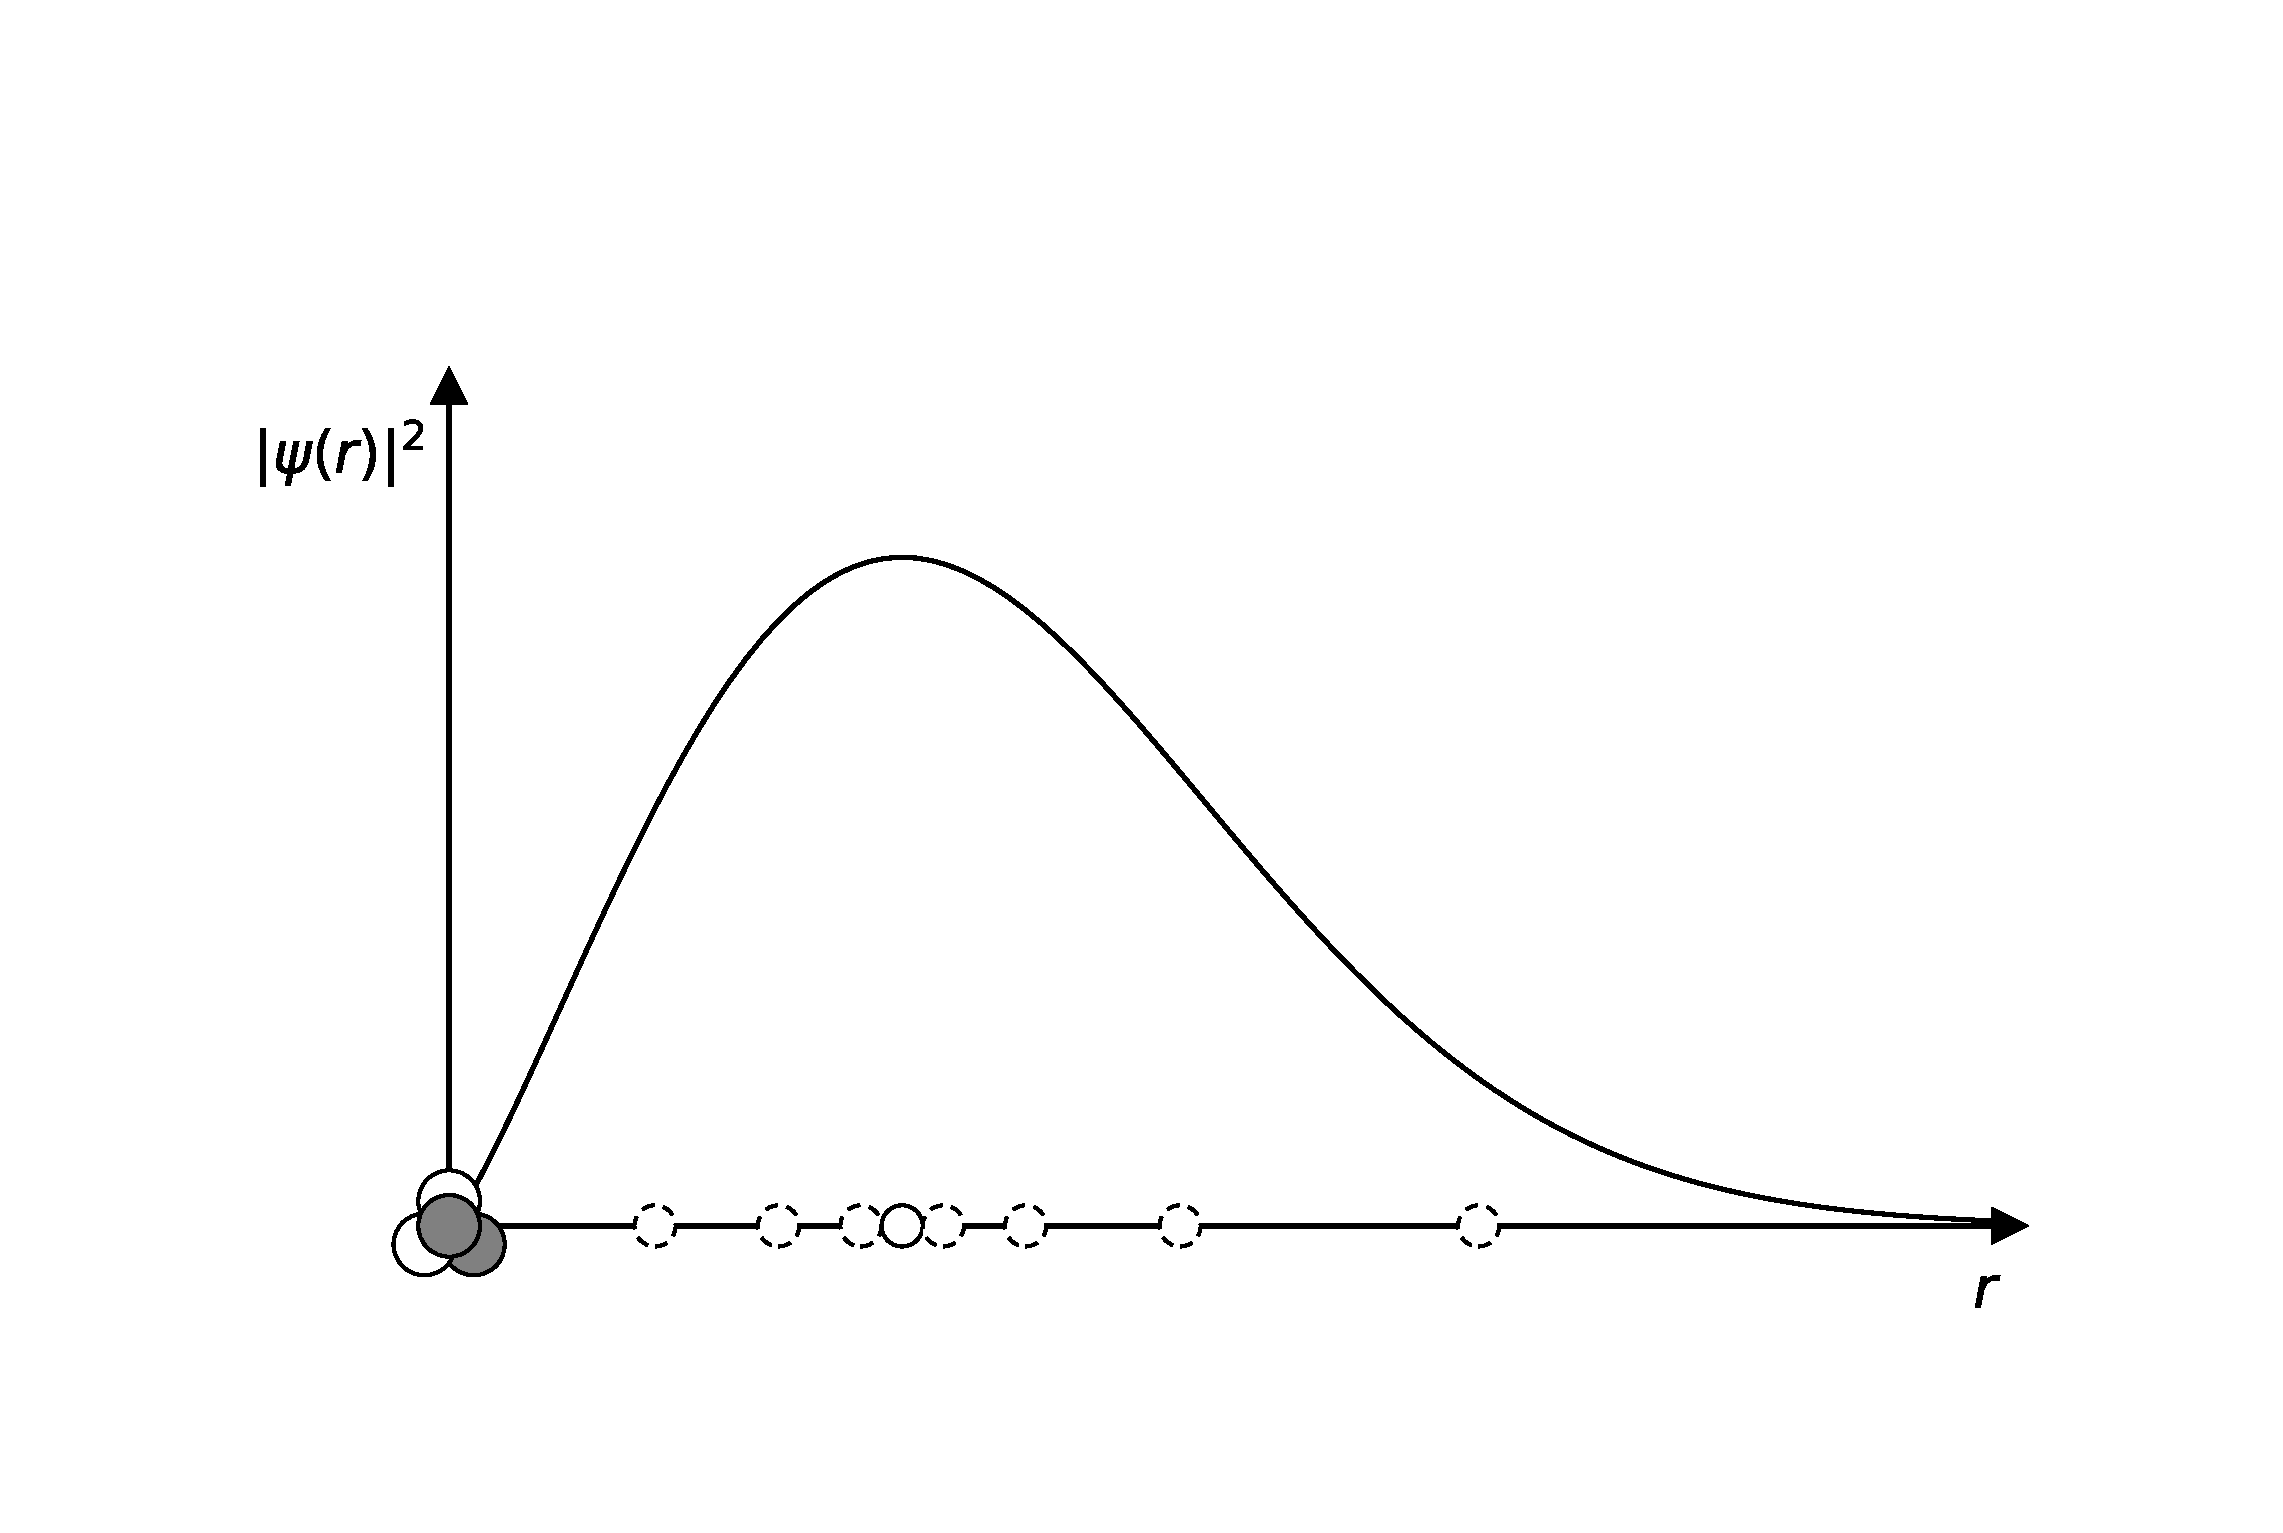
\includegraphics[scale=0.4]{images/radial_prob}
   \caption{Сферически симметричная плотность вероятности местонахождения электрона атома гелия как функция расстояния $r$ до ядра. Электрон может находиться не только в наиболее вероятном месте - точке максимума плотности, но и вообще в любом месте, хотя и с меньшей вероятностью.}
   \label{fig:radial_prob}
\end{figure}


------------------------ IDEAS ------------------------ 

По словам Эйнштейна, ``воображение важнее знания, так как знание ограничено''.
В XX веке теории об атоме предстояло пережить... что даже воображение не всегда справлялось...


Атом вполне может приобретать или терять электроны, получая таким образом заряд и становясь \textit{ионом}.
Порцессы ионизации в ядерных реакциях нас не 



атомы - интуиция еще со времен древних греков, но дальше - перерыв почти на x000 лет связанный с тем, что увидеть объект своих измышлений уже не возможно.
прорыв - с появлением соответсвующих средств измерений, но тут ученых ждал очень большой сбрприз
до этого схема научных открытий в большинстве своем состояла в следующем - смотрели, измеряли, придумывали теорию основнную на уже известных аналогиях, потом совершенствовали приборы, и снова смотрели и придумывали анлогию и т.п.
в атомной физике известных аналогий не нашлось. Наблюдения зачастую в корне противоречили известным фактам о макромире. Любая попытка смотреть на макро-аналогии заканчивалась появлением множества противоречий теории с экспериментом и в конце концов полным провалом 


физика - ранее умение делать открытия зависело от того, насколько наблюдателен был ученый, насколько хорошо он умел проводить параллели между уже известными ялениями и только изучаемыми.
Движения огромных небесных тел описывалось исходя из аналогичных движений, которые можно было повторять в удобном масштабе в своей алборатории и т.п. [еще примеры]
Новая физика потребовала от ученых вообразить нечто не имевшее аналогов с ранее изученным в принципе. 
Это восхищало даже далеких от физики современников.
В математике такие штуки привыкли проворачивать довольно давно. 
Стефан Банах, один из создателей современной математики в ее [современном] виде, говорил "Хорошие математики видят аналогии, лучшие могут видеть аналигии между аналогиями". Сам он, безусловно, был одним из лучших.

 
слова "теория относительности", "квантовая механика" носились в воздухе. Их можно было слышать  понимающих и истолковыва

----------------------------



https://ru.wikipedia.org/wiki/%D0%AD%D0%BB%D0%B5%D0%BA%D1%82%D1%80%D0%BE%D0%BD%D0%BD%D0%B0%D1%8F_%D0%BF%D0%BB%D0%BE%D1%82%D0%BD%D0%BE%D1%81%D1%82%D1%8C
{
В качестве модели состояния электрона в атоме, в квантовой механике принято представление об электронном облаке, плотность соответствующих участков которого пропорциональна вероятности нахождения там электрона.

Электронное облако часто изображают в виде граничной поверхности. При этом обозначение электронной области при помощи точек опускают. Пространство вокруг ядра, в котором наиболее вероятно пребывание электрона, называют атомной орбиталью (смысл которого вытекает из волнового уравнения Шрёдингера).

Применяются графические изображения распределения электронной плотности относительно ядра.

Кривая радиального распределения вероятности показывает, что электрон находится в тонком концентрическом шаровом слое радиуса r толщины dr вокруг ядра атома водорода[1].

Проекция максимума кривой соответствует боровскому радиусу alpha_0=0,53 A_with_circle.

Во многих случаях для решения уравнения Шрёдингера используют различные приближения. Вероятностную (статистическую) интерпретацию волновой функции разработал Макс Борн. В 1954 году М.Борн удостоен Нобелевской премии по физике с формулировкой «За фундаментальные исследования в области квантовой механики, особенно, за статистическую интерпретацию волновой функции.»
}

https://ru.wikipedia.org/wiki/%D0%A1%D1%82%D0%B0%D1%82%D0%B8%D1%81%D1%82%D0%B8%D1%87%D0%B5%D1%81%D0%BA%D0%B0%D1%8F_%D0%B8%D0%BD%D1%82%D0%B5%D1%80%D0%BF%D1%80%D0%B5%D1%82%D0%B0%D1%86%D0%B8%D1%8F_%D0%B2%D0%BE%D0%BB%D0%BD%D0%BE%D0%B2%D0%BE%D0%B9_%D1%84%D1%83%D0%BD%D0%BA%D1%86%D0%B8%D0%B8
{
М. Борн вспоминал:
Он (Шрёдингер) рассматривал электрон не как частицу, но как некоторое распределение плотности, которое давалось квадратом его волновой функции |ψ|².

Он считал, что следует полностью отказаться от идеи частиц и квантовых скачков, и никогда не сомневался в правильности этого убеждения. Я, напротив, имел возможность каждодневно убеждаться в плодотворности концепции частиц, наблюдая за блестящими опытами Франка по атомным и молекулярным столкновениям, и был убеждён, что частицы не могут быть упразднены. Следовало найти путь к объединению частиц и волн. Я видел связующее звено в идее вероятности…
}


